\section[Wykład 7: 20-IV-2017 - Temat: Łańcuchy Markowa]{Temat: Łańcuchy Markowa}
Mottem a zarazem prezentacją wykładu jest ,,gra w życie'' \url{https://bitstorm.org/gameoflife/}

\subsection{,,Rozgrzewka''}
\begin{example*}\label{exa:student}
Student błądzi między Biblioteką, Wykładem a Ćwiczeniami i co 5 minut decyduje co robić dalej?\\
Graf możliwych decyzji studenta poniżej:
\begin{figure}[H]
\centering
\begin{tikzpicture}[shorten >=1pt, auto, node distance=3cm, ultra thick,main node/.style={circle,draw,minimum size=.4cm,inner sep=0pt}]
\begin{scope}[every node/.style={font=\sffamily\large\bfseries}]
\node [main node](v1) at (2,3) {B};
\node [main node](v2) at (0,0) {C};
\node [main node](v3) at (4,0) {W};
\end{scope}
\path 
	(v1) edge [->] node {$\sfrac{1}{4}$} (v2)
    	 edge [->,bend left] node {$\sfrac{1}{4}$} (v3)
    	 edge [loop above]   node {$\sfrac{1}{2}$} (v1)
    (v2) edge [->,bend left] node {$\sfrac{2}{3}$} (v1)
    	 edge [->] node {$\sfrac{1}{3}$} (v3)
    (v3) edge [->] node {$\sfrac{2}{3}$} (v1)
    	 edge [->,bend left] node {$\sfrac{1}{3}$} (v2)
         ;
\end{tikzpicture}
\end{figure}
\textbf{Start:} Biblioteka, czyli:
\begin{description}
\item[$X_0$] miejsce początkowe
\item[$x_1$] miejsce w pierwszym kroku
\item[$x_2$] miejsce w drugim kroku
\end{description}
$\mathsf{Pr}(X_0=B)=1$
$$\begin{array}{l|lll}
 & B & C & W \\ \hline
0 & 1 & 0 & 0 \\ \hline
1 & \sfrac{1}{2} & \sfrac{1}{4} & \sfrac{1}{4} \\ \hline
2 & \sfrac{7}{12} & \sfrac{5}{24} & \sfrac{5}{24} \\ \hline
\end{array}$$
$\mathsf{Pr}(X_2=B)=\frac{1}{2}*\frac{1}{2}+\frac{1}{4}*\frac{2}{3}+\frac{1}{4}*\frac{2}{3}=\frac{7}{12}$
\begin{description}
\item[$p_{ij}(x)$] $\rightarrow$ prawdopodobieństwo przejścia w jednym kroku z obiektu $i$ do obiektu $j$ w $x$ krokach.
\end{description}
Dla przykładu wyżej: $p_{BB}(2)=p_{BB}*p_{BB}+p_{BW}*p_{WB}+p_{BC}*p_{CB}$ 
$$\mathbb{P}= \bordermatrix{~ & B & C & W \cr
                  B & \sfrac{1}{2} & \sfrac{1}{4} & \sfrac{1}{4} \cr
                  C & \sfrac{2}{3} & 0 & \sfrac{1}{3}\cr
                  W & \sfrac{2}{3} & \sfrac{1}{3} &0 \cr}$$
\end{example*}

\subsection{Definicje}
\begin{definition}[Macierz stochastyczna]
Macierz $A=[a_{ij}]$ rozmiaru $n\times n$ nazywamy \textbf{macierzą stochastyczną} jeśli:
\begin{align*}
a_{ij}\geq 0 \text{ dla każdego }i,j\\
\sum_j a_{ij}=1 \text{ dla każdego } i 
\end{align*}
\end{definition}
\begin{definition}[(nieformalna) Łańcuchy Markowa]
Proces losowy, którego pozycja w następnym kroku zależy od obecnej (teraźniejszej) pozycji.
\end{definition}
\begin{definition}[(foramlna) Łańcuchy Markowa]
Niech $S$ będzie skończonym, niepustym zbiorem.\\
Niech macierz $\mathbb{P}=[p_{ij}]_{i,j\in S}$ będzie macierzą stochastyczną.\\
Niech $X_0, X_1, X_2,...$ będą zmiennymi losowymi: $X: \Omega \rightarrow S$.\\
Ciąg $$(X_i)_{i=0}^\infty$$ nazywamy \textbf{Łańcuchem Markowa} macierz przejścia $\mathbb{P}$, gdy:
\begin{enumerate}[label=\arabic*.]
\item Warunek / Własność Markowa:
\begin{align*}
&\mathsf{Pr}(X_t=s_t|X_{t-1}=s_{t-1},X_{t-2}=s_{t-2},...,X_0=s_0)=\\
&\mathsf{Pr}(X_t=s_t|X_{t-1}=s_{t-1})
\end{align*} dla $t\in \mathbb{N}_+$ i $s_t, s_{t-1},...,s_0\in S$\footnote{O ile mają sens, czytaj: $\mathsf{Pr}(X_t=s_t|X_{t-1}=s_{t-1},...,X_0=s_0)>0$}
\item $$\mathsf{Pr}(X_t=s_t|X_{t-1}=s')=p_{ss'}$$ dla $t\in \mathbb{N}_+$ i $s,s'\in S$\footnote{o ile $\mathsf{Pr}(X_{t-1}=s')>0$}
\end{enumerate}
Jest to definicja \textbf{Skończonego jednorodnego Łańcuchu Markowa} czytaj: $|S|<\infty$, gdzie 
\begin{description}
\item[$S$] to przestrzeń stanów Łańcuchów Markowa
\item[$X_0$] rozkład początkowy Łańcuchów Markowa
\end{description}
\end{definition}

\begin{example*} 
Ciąg dalszy ,,dylematu studenta'' z strony \pageref{exa:student}
\begin{align*}
&S=\{B,C,W\}\\
&X_i \rightarrow \text{ położenie (stan) Studenta po }i\text{ krokach}
&\mathbb{P}=\begin{bmatrix}
\sfrac{1}{2} & \sfrac{1}{4} & \sfrac{1}{4} \\
\sfrac{2}{3} & 0 & \sfrac{1}{3}\\
\sfrac{2}{3} & \sfrac{1}{3} &0 
\end{bmatrix}\\
&(X_i)_{i=0}^\infty \text{ jest Łańcuchem Markowa macierzy przejścia }\mathbb{P}
\end{align*}
\end{example*}
\begin{example*} 
Dwie osoby Ala i Franek rzucają na przemiennie monetą. Ala wygrywa, gdy nastąpi sekwencja $OOR$, Franek wygrywa, gdy nastąpi sekwencja $ROR$. 
\begin{itemize}
\item[] Kto ma większe szanse na wygraną? 
\item[] Ile średnio czasu trwa gra?
\end{itemize}
Próbny rozwiązania:
\begin{enumerate}[label=Próba \Roman*.]
\item $S=\{O,R\}$
\begin{description}
\item[$X_i$] co wypadło w $i$ tym rzucie
\item[$(X_i)_{i=0}^\infty$] Łańcuch Markowa o macierzy:
$$\mathbb{P}=\begin{bmatrix}
\sfrac{1}{2}&\sfrac{1}{2}\\\sfrac{1}{2}&\sfrac{1}{2}
\end{bmatrix}$$
\end{description}
\textbf{PUDŁO} - nie oddaje ducha gry

\item $S=\{O,R,W_A,W_F\}$
\begin{align*}
&X_i=\left\{\begin{matrix}
O/R & \text{ Nie ma zwycięzcy }\\
W_A & \text{ Wygrała Ala w }i\text{ tym rzucie} \\
W_F & \text{ Wygrał Franek w }i\text{ tym rzucie} \\
\end{matrix}
\right.\\
&(X_i)_{i=0}^\infty \text{to nie Łańcuch Markowa, gdyż: }\\
&\mathsf{Pr}(X_3=O|X_2=R,X_1=O,X_0=R)=0\\
&\mathsf{Pr}(X_3=O|X_2=R,X_1=R,X_0=R)=0
\end{align*}

\item $S=\{O,R,OO,RO,W_A,W_F\}$\\
$X_i$ to stan w którym jest gra po $i$ rzutach
\begin{figure}[H]
\centering
\begin{tikzpicture}[shorten >=1pt, auto, node distance=3cm, ultra thick,main node/.style={circle,draw,minimum size=.4cm,inner sep=0pt}]
\begin{scope}[every node/.style={font=\sffamily\large\bfseries}]
\node [main node](v1) at (0,0) {R};
\node [main node](v2) at (2,0) {RO};
\node [main node](v3) at (2,2) {OO};
\node [main node](v4) at (0,2) {O};
\node [main node](v5) at (4,0) {$W_F$};
\node [main node](v6) at (4,2) {$W_A$};
\end{scope}
\path 
	(v1) edge [->] node {$\sfrac{1}{2}$} (v2)
    	 edge [loop below]   node {$\sfrac{1}{2}$} (v1)
    (v2) edge [->] node {$\sfrac{1}{2}$} (v3)
    	 edge [->] node {$\sfrac{1}{2}$} (v5)
    (v3) edge [loop above] node {$\sfrac{1}{2}$} (v3)
    	 edge [->] node {$\sfrac{1}{2}$} (v6)
    (v4) edge [->] node {$\sfrac{1}{2}$} (v3)
    	 edge [->] node {$\sfrac{1}{2}$} (v1)
         ;
\end{tikzpicture}
\end{figure}
To jest Łańcuch Markowa\footnote{Moim zadaniem Franek powinien się zbuntować gra serio NOT FAIR}
\end{enumerate}
\end{example*}

\begin{fact*}
$\mathsf{Pr}(t)$ opisuje macierz $\mathbb{P}^t$
\end{fact*}

\begin{example*}
Ciąg dalszy studenta ze strony \pageref{exa:student}.
\begin{align*}
&\mathbb{P}=\begin{bmatrix}
\sfrac{1}{2} & \sfrac{1}{4} & \sfrac{1}{4} \\
\sfrac{2}{3} & 0 & \sfrac{1}{3}\\
\sfrac{2}{3} & \sfrac{1}{3} &0 
\end{bmatrix}\\
&\mathbb{P}^2=\begin{bmatrix}
\sfrac{1}{2} & \sfrac{1}{4} & \sfrac{1}{4} \\
\sfrac{2}{3} & 0 & \sfrac{1}{3}\\
\sfrac{2}{3} & \sfrac{1}{3} &0 
\end{bmatrix}\begin{bmatrix}
\sfrac{1}{2} & \sfrac{1}{4} & \sfrac{1}{4} \\
\sfrac{2}{3} & 0 & \sfrac{1}{3}\\
\sfrac{2}{3} & \sfrac{1}{3} &0 
\end{bmatrix}=\begin{bmatrix}
\sfrac{42}{72} & \sfrac{15}{72} & \sfrac{15}{72} \\
\sfrac{40}{72} & \sfrac{20}{72} & \sfrac{12}{72}\\
\sfrac{40}{72} & \sfrac{12}{72} & \sfrac{20}{72}
\end{bmatrix}\\
&\bar{p}(1)=\begin{bmatrix}
\sfrac{1}{2} & \sfrac{1}{4} & \sfrac{1}{4}
\end{bmatrix}\\
&\bar{p}(2)=\begin{bmatrix}
\sfrac{42}{72} & \sfrac{15}{72} & \sfrac{15}{72}
\end{bmatrix}
\end{align*}
\end{example*}

Dla $(X_i)_{i=0}^\infty$ $\bar{p}(t)$ to wektor opisujący rozkład zmiennej po $t$ krokach.

\begin{fact*}
$\mathbb{P}$ i rozkład zmiennej losowej początkowej ($X_0$) jednoznacznie określa rozkład $X_t$\\
\textbf{Przepis:}
\begin{enumerate}[label=\arabic*.]
\item $\bar{p}(t)=\bar{p}(0)*\mathbb{P}^t$
\item $\bar{p}(t)=\bar{p}(t-1)*\mathbb{P}$
\end{enumerate}
\end{fact*}

